\section{Results and Discussion} \label{sec:results}

Here, we report a series of benchmarks that evaluate the viability of our proposed approaches to harness the CS-2 accelerator for digital evolution simulations and extract phylogenetic records from said simulations.
First, we compare the performance characteristics of new surface-oriented hereditary stratigraphy methods against preceding column-based implementation to determine the extent to which they succeed in streamlining runtime operation.
%For assessment of  we refer the reader to related work TODOCITE.
Then, we benchmark phylogeny-tracked WSE genetic algorithm implementation.
To assess the runtime overhead of surface-based tracking, we compare against benchmarking results with phylogenetic tracking disabled.
Finally, we validate the credibility of the presented end-to-end annotation-to-reconstruction pipeline by reviewing the clade structure from varying-duration emulated WSE evolutionary runs.
% Finally, we show example phylogenies generated from on-hardware simulations under different selection pressure conditions and test the capability of inference from extracted phylogenetic information to detect differing selection pressure conditions.

% TODO transplant this into the other paper
% \subsection{Reconstruction Quality of New Surface Algorithms}

% \begin{figure*}
  \centering
  \includegraphics[width=\textwidth]{binder-reconstruction-quality/binder/surf-vs-col/outplots/surf-vs-col-table}
  \caption{%
   \textbf{Comparison of reconstruction accuracies from column- and surface-based annotations.}
    Color coding represents non-parametric difference between accuracy measures, with red indicating superior surface performance and blue indicating superior column performance.
    Left column shows tilted retention policies, and right column shows steady retention policies.
    For heatmap charts, +'s indicate small, medium, and large effect sizes using the Cliff's delta statistic and *'s indicate statistical significance at $\alpha = 0.05$ via Mann-Whitney U test.
  }
  \label{fig:col-vs-surf}
\end{figure*}


% Figure \ref{fig:col-vs-surf} compares reconstruction quality for surface algorithms against their corresponding column implementation.
% We did this by using a simple simulation to generate phylogenies under different conditions with perfect tracking, then simulating heritage of hstrat annotations down the perfect tree and subsequent reconstruction.
% We could then compare the reconstruction that would have been obtained under approximate tracking to the underlying ground truth.

% To ensure generalizable results, we tested over a large number of evolutionary regimes, population sizes, instrumentation sizes, and instrumentation fingerprint sizes.
% Each row in Figure \ref{fig:col-vs-surf} represents a distinct combination of surveyed conditions.

% We took three measures of reconstruction quality.
% The first measure, triplet distance, is a measure of accuracy --- it is the fraction of triplet tips that are correctly arranged in the reconstruction.
% Whereas this metric considers polytomies as distinct from separate branching events, our second measure is a lax variant of triplet distance that does not penalize penalties introduced into the reconstruction (i.e., due to uncertainty about branching order) or over-resolution of true polytomies into more nodes in the reconstruction.
% Finally, we also include inner node count, which provides a measure of the amount of detail achieved by reconstructions.
% Higher inner node count indicates that fewer branching events are being lumped together into polytomies due to insufficient information to differentiate them.
% This metric is only applicable to scenarios with fingerprint sizes larger than one bit (i.e., a byte), which are capable of generating non-bifurcating trees.

% The data tell two clear stories:
% \begin{enumerate}
% \item surface tilted algorithms create higher-quality reconstructions than column-based tilted algorithms and
% \item surface column algorithms create lower-quality reconstructions than column-based column algorithms.
% \end{enumerate}

% The surface tilted performs significantly best in 14 / 48 scenarios for triplet distance, 9 / 48 for lax triplet distance, and all scenarios where inner node count is applicable.
% It performs significantly worse in no scenarios.

% The surface steady performs significantly worse in 11 / 48 scenarios for triplet distance, in 1/48 scenarios for lax triplet distance, and 4/12 scenarios for inner node loss.
% The surface steady performs significantly better than the column in no scenarios.

% The performance advantage of surface-tilted is likely because the surface-based algorithms can make better use of available space --- every site is always in use to store a fingerprint.
% In contrast, under the column-based approach, some fraction of the available space is typically unused because of difficulty predicting the order with which sites will need to be eliminated \textit{a priori} and thus eliminating them based on a heuristic (TODO rewrite this sentence).

% The performance detriment of column-steady likely stems from precise control of the column approach to sequence eliminations.
% The surface approach guarantees adherence to the fixed resolution qualities provided by the column approach, but the process of degrading from one spacing to the next double-width spacing is slightly more irregular on account of the additional consideration of being mapped onto the surface.
% Unlike the tilted algorithm, the steady column algorithm does not have difficulty filling available space.

% Recent work indicates that tilted policies should be preferred for better reconstruction accuracy in most cases, except where there are extreme factors promoting phylogenetic richness.
% Thus, degraded reconstruction performance from the steady surface is not much of a concern because the steady policy is not expected to be used frequently in practice.
% So, in addition to being capable of being implemented in a broader range of device contexts (not needing memory allocation or rich data structures) and being faster to calculate (discussed next), the surface-based approach can provide higher-quality phylogenetic reconstructions.

\subsection{Surface Algorithm Benchmark}

\begin{figure*}
  \centering
  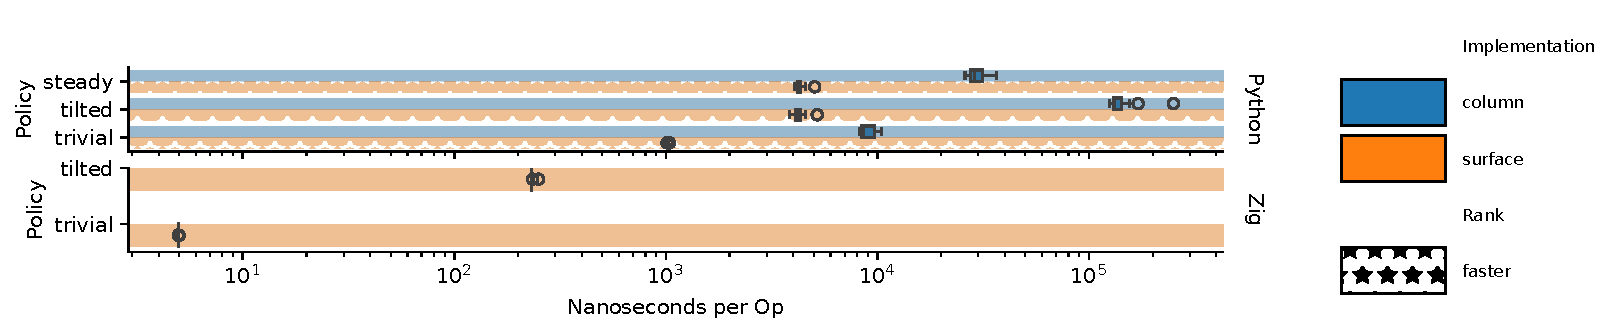
\includegraphics[width=\textwidth]{binder-wafer-scale/binder/teeplots/all=false+hue=implementation+orient=h+row=language+score=nanoseconds-per-op+viz=peckplot+x=nanoseconds-per-op+y=policy+y-group=outer+ext=}

\vspace{-2.5ex}

  \caption{%
    \textbf{Hereditary stratigraphy algorithm benchmarks.}
    \footnotesize
    Comparison of per-generation operation time for column- and surface-based steady and tilted retention policies, lower is better.
  Top and bottom panels show Python and Zig implementations, respectively.
    Trivial is a simple harcoded retention decision, provided as a baseline control.
    Background hatching indicates significant outcome (Mann-Whitney U test; $n=20$).
  }
  \label{fig:benchmarking}
  \vspace{-0.2in}
\end{figure*}


We performed microbenchmark experiments to test computational efficiency gains from new surface-based algorithms.
Trials measured the per-generation execution time of repeated sequential updates to one annotation with capacity for 64 differentia. % TODO check this
Benchmarks were conducted both using Python, for comparability with existing column algorithm implementations, and Zig, to assess performance in absolute terms under compiler optimization.
Figure \ref{fig:benchmarking} overviews results.

% Due to limited completed implementations of compiled-language algorithms, we performed the bulk of benchmarking using the Python implementations.
% However, in the process of porting the tilted surface algorithm over to Cerebras Software Language, we did create an implementation of that algorithm in Zig which is a compiled language and is capable of compiler optimizations.
% We augment the Python with a benchmark of this algorithm.

% https://github.com/mmore500/hstrat-surface-concept/blob/51d636d768d474fc5148b9fcaa199c1b7776e915/benchmark.ipynb
Python implementations of the surface tilted and steady algorithms both took around 4.2 microseconds per operation (SEM approx. 50; $n=20$).
For context, this was about $4\times$ the measured time for a surface placement using a trivial calculation (SEM approx. 0.05; $n=20$).
As expected, column implementations of steady and tilted fared much worse, taking about $7\times$ and $34\times$ the execution time per operation compared to the surface operations.
In both cases, surface implementations significantly outperformed their column counterparts (Mann-Whitney U test, $\alpha = 0.05$).
It should be noted that these results reflect an intrinsic performance penalty due to interpreter overhead of Python evaluation.
However, comparisons among these Python implementations are nonetheless informative because all are on equal footing in this regard.
% While Python is an interpreted language and the Python-implemented algorithms weren't specifically implemented to maximize performance and suffer an intrinsic performance penalty due to that, the algorithms were all on the same footing and
% We use the ``optimize''' flag to strip superfluous safety checks.

% https://github.com/mmore500/wse-sketches/blob/d4ab0155f63ff5809f8eeca1169ad9b272c30a68/binder/benchmark.ipynb
Zig microbenchmarks clock tilted surface annotation updates at 233 ns per operation (SEM 0.9; $n=20$).
For context, this time a little more than twice the amount of time required for a main memory access in contemporary computing hardware \citep{markus2022memory}.
Our results measure the operation at $47\times$ the measured time for a trivial placement calculation (SEM 0.2; $n=20$).
Steady results are not included in this comparison due to a Zig implementation not yet being completed.

Low-hanging speedups and optimizations exist to further improve per-operation surface update performance achieved in practice.
Half of update operations on surfaces with single-bit differentia can be skipped entirely, owing to 50\% probability that randomization fails to change a stored differentia value.
Further, simulations with synchronous or near-synchronous generations can cache calculated surface-placement indices, meaning they would only need to be computed once for an entire subpopulation.
Another possibility is to coarsen temporal resolution, only updating annotations at intervals every $n$th generation.

\subsection{WSE Island-model GA Benchmark}

Next, we sought to characterize the performance of our island model genetic algorithm implementation on WSE hardware and estimate the magnitude of simulation that might be achieved with on-device execution.
We used per-PE cycle counters in emulation to test the amount of real-time elapsed over the course of a 40 generation-cycle simulation.
We tested using a $3\times3$ PE collective with the tagged 3-word genome and a per-PE population size of 32, applying a tilted hereditary stratigraphy every generation.

PEs completed a mean of 24,138 generation-cycles per second (SEM 99; $n=9$).
As an indicator of inter-PE exchange throughput, each PE immigrated a mean of 118 genomes (SEM 11; $n=9$) over 40 elapsed generation-cycles.

% https://osf.io/tf89g
What scale of simulation does this performance imply at full scale on CS-2 hardware?
Across eight 1 million generation on-device tracking-enabled trials described below, we measured a mean generation rate of 17,688 hz for 562,500 PEs ($750\times750$ rectangle) with runtimes slightly below one minute.
As a point of comparison, eight trials trials conducted with 1,600 PEs ($40\times40$) yielded a similar mean generation rate of 17,734 hz.

Multiplied out to a full day, a 17 kHz turnover rate would elapse around 1.5 billion generations.
With 32 individuals hosted per each of 850,000 PEs, the net population size would sit around 27 million at full CS-2 wafer scale.
(Note, though, that available on-chip memory could support thousands of our very simple agents per PE, raising the potential for a net population size on the order of a billion agents.)
% 24,000 * 850,000 * 60 * 60 * 24 * 32 ---> ?? quadrillion
A naive extrapolation estimates on the order of a quadrillion agent replications could be achieved hourly at full wafer scale for such a very simple model.
We look forward to conducting more thorough benchmarking and scaling experiments in future work.
%The barebones simplicity of the model should also be noted.

Recall that these figures are inclusive of phylogenetic tracking.
How fast does simulation run without hereditary stratigraphy instrumentation?
Using the hardware emulator, we repeated our benchmark using one-word genomes stripped of all instrumentation.
Under these conditions, PEs completed a mean of 47,175 generations per second (SEM 220; $n=20$)
As before, over the course of simulation, each PE immigrated on average 118 genomes (SEM 12; $n=12$).

These timings indicate cost of phylogeny tracking as approximately equivalent to that of the other aspects of simulation, combined.
Given the highly minimalistic nature of the agent model and selection process, this result is highly promising.
In actual use, most experiments will likely involve a much more sophisticated agent model and, thus, the relative overhead of tracking will diminish significantly.
It is additionally worthwhile to note that caching and coarsening strategies discussed above have not yet been applied, which may reduce performance penalty of tracking considerably.

% https://github.com/mmore500/wse-sketches-mirror/actions/runs/8590107511/job/23537207835
% from https://github.com/mmore500/wse-sketches-mirror/commit/3a1bf8e9f2820a38cb7387a7624a86361485174b
% ASYNC_GA_GENOME_FLAVOR genome_purifyingplus
% ASYNC_GA_GLOBAL_SEED 0
% ASYNC_GA_NCYCLE_AT_LEAST 40
% ASYNC_GA_MSEC_AT_LEAST 0
% ASYNC_GA_TSC_AT_LEAST 0
% INFO: Using SIF: /home/runner/cerebras/bin/cbcore_sdk-202311111408-10-4a54bce5.sif
% INFO: User's specified CSL_IMPORT_PATH=
% NOTE: CSL_IMPORT_PATH accepts colon separated list of paths generated by 'realpath <path>'
% INFO:    Environment variable SINGULARITYENV_CSL_SUPPRESS_SIMFAB_TRACE is set, but APPTAINERENV_CSL_SUPPRESS_SIMFAB_TRACE is preferred
% compile successful
% Updated 1 path from the index
% CS_PYTHON cs_python
% INFO: Using SIF: /home/runner/cerebras/bin/cbcore_sdk-202311111408-10-4a54bce5.sif
% INFO:    Environment variable SINGULARITYENV_CSL_SUPPRESS_SIMFAB_TRACE is set, but APPTAINERENV_CSL_SUPPRESS_SIMFAB_TRACE is preferred
% whoami ===============================================================
% [[0 3 6]
%  [1 4 7]
%  [2 5 8]]
% whereami x ===========================================================
% [[0 1 2]
%  [0 1 2]
%  [0 1 2]]
% whereami y ===========================================================
% [[0 0 0]
%  [1 1 1]
%  [2 2 2]]
% cycle counter =======================================================
% [[40 40 40]
%  [40 40 40]
%  [40 40 40]]
% recv counter N ========================================================
% [[ 1  1  1]
%  [ 9 13 11]
%  [15 12 12]]
% recv counter S ========================================================
% [[ 7  9  8]
%  [10 11  9]
%  [ 1  1  1]]
% recv counter E ========================================================
% [[12 11  1]
%  [12 13  1]
%  [ 9 13  1]]
% recv counter W ========================================================
% [[ 1 11  9]
%  [ 1  7  9]
%  [ 1 10 11]]
% recv counter sum =====================================================
% [21, 32, 19, 32, 44, 30, 26, 36, 25]
% np.mean(recvSum)=29.444444444444443 np.std(recvSum)=7.304657739508267 sps.sem(recvSum)=2.5825865109265465
% send counter N ========================================================
% [[ 0  0  0]
%  [24 32 34]
%  [40 46 34]]
% send counter S ========================================================
% [[38 50 46]
%  [58 50 48]
%  [ 0  0  0]]
% send counter E ========================================================
% [[44 32  0]
%  [24 32  0]
%  [40 46  0]]
% send counter W ========================================================
% [[ 0 50 46]
%  [ 0 50 48]
%  [ 0 36 48]]
% send counter sum =====================================================
% [82, 132, 92, 106, 164, 130, 80, 128, 82]
% np.mean(sendSum)=110.66666666666667 np.std(sendSum)=27.744869395579748 sps.sem(sendSum)=9.809292646374773
% tscControl values ====================================================
% [30064968187, 30064968187, 30064968187, 30064968187, 30064968187, 30064968187, 30064968187, 30064968187, 30064968187]
% tscStart values ======================================================
% [2220, 2222, 2731, 2731, 1716, 2738, 3241, 3243, 3237]
% tscEnd values ========================================================
% [1414233, 1414662, 1406657, 1388294, 1438771, 1433887, 1412082, 1403426, 1390454]
% tsc diffs ============================================================
% --------------------------------------------------------------- ticks
% [1412013, 1412440, 1403926, 1385563, 1437055, 1431149, 1408841, 1400183, 1387217]
% np.mean(tsc_ticks)=1408709.6666666667 np.std(tsc_ticks)=16415.157825754963 sps.sem(tsc_ticks)=5803.63470641938
% -------------------------------------------------------------- seconds
% [0.0016611917647058824, 0.0016616941176470588, 0.0016516776470588235, 0.0016300741176470588, 0.0016906529411764705, 0.0016837047058823528, 0.00165746, 0.0016472741176470588, 0.00163202]
% np.mean(tsc_sec)=0.0016573054901960784 np.std(tsc_sec)=1.9311950383241098e-05 sps.sem(tsc_sec)=6.827805536963963e-06
% ---------------------------------------------------- seconds per cycle
% [4.152979411764706e-05, 4.154235294117647e-05, 4.129194117647059e-05, 4.075185294117647e-05, 4.226632352941176e-05, 4.209261764705882e-05, 4.1436499999999995e-05, 4.1181852941176466e-05, 4.0800500000000003e-05]
% np.mean(tsc_cysec)=4.143263725490196e-05 np.std(tsc_cysec)=4.827987595810268e-07 sps.sem(tsc_cysec)=1.7069513842409884e-07
% ---------------------------------------------------------- cycle hertz
% [24079.09842189838, 24071.81897992127, 24217.800653310787, 24538.761499837972, 23659.498070707108, 23757.135001317125, 24133.312417795907, 24282.540210815303, 24509.50356000539]
% np.mean(tsc_cyhz)=24138.829868401026 np.std(tsc_cyhz)=280.43062795032466 sps.sem(tsc_cyhz)=99.14719933803819
% --------------------------------------------------------- ns per cycle
% [41529.79411764706, 41542.35294117647, 41291.94117647059, 40751.852941176476, 42266.32352941176, 42092.61764705882, 41436.49999999999, 41181.85294117647, 40800.5]
% np.mean(tsc_cyns)=41432.63725490196 np.std(tsc_cyns)=482.7987595810264 sps.sem(tsc_cyns)=170.6951384240987
% fitness =============================================================
% [[0.00316905 0.00565182 0.0022315 ]
%  [0.00687918 0.00742484 0.00589414]
%  [0.00582986 0.0057458  0.00379858]]


% https://github.com/mmore500/wse-sketches-mirror/actions/runs/8590107511/job/23537207835
% from https://github.com/mmore500/wse-sketches-mirror/commit/3a1bf8e9f2820a38cb7387a7624a86361485174b
% CSLC cslc
% ASYNC_GA_GENOME_FLAVOR genome_purifyingstripped
% ASYNC_GA_GLOBAL_SEED 0
% ASYNC_GA_NCYCLE_AT_LEAST 40
% ASYNC_GA_MSEC_AT_LEAST 0
% ASYNC_GA_TSC_AT_LEAST 0
% INFO: Using SIF: /home/runner/cerebras/bin/cbcore_sdk-202311111408-10-4a54bce5.sif
% INFO: User's specified CSL_IMPORT_PATH=
% NOTE: CSL_IMPORT_PATH accepts colon separated list of paths generated by 'realpath <path>'
% INFO:    Environment variable SINGULARITYENV_CSL_SUPPRESS_SIMFAB_TRACE is set, but APPTAINERENV_CSL_SUPPRESS_SIMFAB_TRACE is preferred
% compile successful
% Updated 1 path from the index
% CS_PYTHON cs_python
% INFO: Using SIF: /home/runner/cerebras/bin/cbcore_sdk-202311111408-10-4a54bce5.sif
% INFO:    Environment variable SINGULARITYENV_CSL_SUPPRESS_SIMFAB_TRACE is set, but APPTAINERENV_CSL_SUPPRESS_SIMFAB_TRACE is preferred
% whoami ===============================================================
% [[0 3 6]
%  [1 4 7]
%  [2 5 8]]
% whereami x ===========================================================
% [[0 1 2]
%  [0 1 2]
%  [0 1 2]]
% whereami y ===========================================================
% [[0 0 0]
%  [1 1 1]
%  [2 2 2]]
% cycle counter =======================================================
% [[40 40 40]
%  [40 40 40]
%  [40 40 40]]
% recv counter N ========================================================
% [[ 1  1  1]
%  [13 11 14]
%  [11  7 11]]
% recv counter S ========================================================
% [[ 9 13  9]
%  [11 13 11]
%  [ 1  1  1]]
% recv counter E ========================================================
% [[11 15  1]
%  [ 7 11  1]
%  [ 7  9  1]]
% recv counter W ========================================================
% [[ 1  7  9]
%  [ 1  9 13]
%  [ 1 11 13]]
% recv counter sum =====================================================
% [22, 36, 20, 32, 44, 39, 20, 28, 26]
% np.mean(recvSum)=29.666666666666668 np.std(recvSum)=8.16496580927726 sps.sem(recvSum)=2.886751345948129
% send counter N ========================================================
% [[ 0  0  0]
%  [38 52 38]
%  [42 52 44]]
% send counter S ========================================================
% [[54 44 56]
%  [44 30 44]
%  [ 0  0  0]]
% send counter E ========================================================
% [[28 38  0]
%  [38 52  0]
%  [42 52  0]]
% send counter W ========================================================
% [[ 0 44 56]
%  [ 0 30 44]
%  [ 0 30 38]]
% send counter sum =====================================================
% [82, 126, 112, 120, 164, 126, 84, 134, 82]
% np.mean(sendSum)=114.44444444444444 np.std(sendSum)=26.192073063391234 sps.sem(sendSum)=9.260296238228726
% tscControl values ====================================================
% [30064968187, 30064968187, 30064968187, 30064968187, 30064968187, 30064968187, 30064968187, 30064968187, 30064968187]
% tscStart values ======================================================
% [1131, 1130, 1644, 1641, 628, 1650, 2151, 2155, 2149]
% tscEnd values ========================================================
% [709983, 736796, 714836, 730020, 721384, 731436, 713213, 730922, 713242]
% tsc diffs ============================================================
% --------------------------------------------------------------- ticks
% [708852, 735666, 713192, 728379, 720756, 729786, 711062, 728767, 711093]
% np.mean(tsc_ticks)=720839.2222222222 np.std(tsc_ticks)=9500.522988853212 sps.sem(tsc_ticks)=3358.9421151183965
% -------------------------------------------------------------- seconds
% [0.0008339435294117647, 0.0008654894117647059, 0.0008390494117647059, 0.0008569164705882353, 0.0008479482352941177, 0.0008585717647058823, 0.0008365435294117647, 0.0008573729411764705, 0.00083658]
% np.mean(tsc_sec)=0.0008480461437908496 np.std(tsc_sec)=1.1177085869239065e-05 sps.sem(tsc_sec)=3.9516966060216395e-06
% ---------------------------------------------------- seconds per cycle
% [2.0848588235294117e-05, 2.1637235294117648e-05, 2.097623529411765e-05, 2.1422911764705883e-05, 2.119870588235294e-05, 2.1464294117647056e-05, 2.0913588235294118e-05, 2.1434323529411762e-05, 2.0914499999999998e-05]
% np.mean(tsc_cysec)=2.1201153594771243e-05 np.std(tsc_cysec)=2.7942714673097676e-07 sps.sem(tsc_cysec)=9.879241515054106e-08
% ---------------------------------------------------------- cycle hertz
% [47964.878423140515, 46216.62547949749, 47672.99689284232, 46678.995413102246, 47172.6908967806, 46589.00006303218, 47815.80227884488, 46654.14323096409, 47813.71775562409]
% np.mean(tsc_cyhz)=47175.427825980936 np.std(tsc_cyhz)=620.9035009060691 sps.sem(tsc_cyhz)=219.52253797657457
% --------------------------------------------------------- ns per cycle
% [20848.58823529412, 21637.235294117647, 20976.23529411765, 21422.91176470588, 21198.70588235294, 21464.294117647056, 20913.58823529412, 21434.323529411762, 20914.499999999996]
% np.mean(tsc_cyns)=21201.15359477124 np.std(tsc_cyns)=279.42714673097595 sps.sem(tsc_cyns)=98.79241515054076
% fitness =============================================================
% [[0. 0. 0.]
%  [0. 0. 0.]
%  [0. 0. 0.]]

\subsection{WSE-to-Reconstruction Validation Experiment}

% We performed extensive tests to be confident in our implementation of phylogenetic tracking for the Cerebras Software Language on the WSE device.
% Extensive other work TODOCITE has validated the underlying hereditary surface algorithm and the reconstruction algorithm.
% We also used extensive unit tests in CSL to ensure the algorithm was working as expected.

Here, we demonstrate phylogenetic reconstructions from the WSE platform and inspect clade structure to qualitatively assess their credibility.
% report the results of an integration test to assess the general validity of .
For these experiments, we tagged genomes with a 16-bit randomly generated identifier at simulation startup, as shown in Supplementary Figure \ref{fig:genome-layout}.
% These identifiers identified clades descending from each founding genome.
Using the hardware emulator, we instantiated populations over a $3\times3$ PE collective for durations of 25, 50, 100, and 250 generation-cycles under drift conditions.
At the end of simulation, phylogenetic reconstruction was conducted using one genome sampled per PE.

\begin{figure*}

\begin{subfigure}[c]{\textwidth}
\begin{minipage}[c]{0.1\textwidth}
    \caption{25 cycles}
    \label{fig:tagged_25}
  \end{minipage}
  \begin{minipage}[c]{0.9\textwidth}
    \includegraphics[width=\textwidth,height=0.8in,trim={0 0.81cm 0 0},clip]{binder-wse-sketches/binder/teeplots/genome=hsurftiltedsticky_tagged+replicate=e4ea2071-8228-42de-af8c-879cedff9ba7+viz=draw-biopython-tree+ext=}
  \end{minipage}
\end{subfigure}

\vspace{-1ex}

\begin{subfigure}[c]{\textwidth}  \begin{minipage}[c]{0.1\textwidth}
    \caption{50 cycles}
    \label{fig:tagged_50}
  \end{minipage}
  \begin{minipage}[c]{0.9\textwidth}
    \includegraphics[width=\textwidth,height=0.8in,trim={0 0.81cm 0 0},clip]{binder-wse-sketches/binder/teeplots/genome=hsurftiltedsticky_tagged+replicate=3d55af5f-7714-45da-9276-e860f46b4d94+viz=draw-biopython-tree+ext=}
  \end{minipage}
\end{subfigure}

\vspace{-1ex}

\begin{subfigure}[c]{\textwidth}
  \begin{minipage}[c]{0.1\textwidth}
    \caption{100 cycles}
    \label{fig:tagged_100}
  \end{minipage}
  \begin{minipage}[c]{0.9\textwidth}
    \includegraphics[width=\textwidth,height=0.8in,trim={0 0.81cm 0 0},clip]{binder-wse-sketches/binder/teeplots/genome=hsurftiltedsticky_tagged+replicate=932aa302-becb-47e8-9712-7f550b02364c+viz=draw-biopython-tree+ext=}
  \end{minipage}
\end{subfigure}

\vspace{-1ex}

\begin{subfigure}[c]{\textwidth}
  \begin{minipage}[c]{0.1\textwidth}
    \caption{250 cycles}
    \label{fig:tagged_250}
  \end{minipage}
  \begin{minipage}[c]{0.9\textwidth}
    \includegraphics[width=\textwidth,height=1in]{binder-wse-sketches/binder/teeplots/genome=hsurftiltedsticky_tagged+replicate=42dbcbb3-b803-41a4-9285-4a450bfad6ed+viz=draw-biopython-tree+ext=}
  \end{minipage}
\end{subfigure}

\caption{%
\textbf{Clade Validation Trial.}
Example phylogenies reconstructed from runs of increasing duration on virtual grid of nine hardware-simulated PEs.
Founding genomes were tagged with random 16-byte identifier values, which were held constant over the course of simulation (Supplementary Figure \ref{fig:genome-layout}).
Color-coding indicates each sampled taxon's founding ancestor according to this identifier value.
Simulation performed under drift conditions.
}
\label{fig:tagged}

\end{figure*}


Figure \ref{fig:tagged} shows reconstructed phylogenies from each duration.
As expected, taxa belonging to the same founding clade (shown by color) are reconstructed as more closely related to each other than to other taxa.
Additionally, and also as expected, the number of distinct remaining founding clades diminishes monotonically with increasing simulation duration.
These consistencies corroborate the general integrity of implemented annotation and reconstruction processes.
Note, however, the incidence of moderate overestimations for relatedness between independently-tagged clades throughout.
As mentioned earlier, and discussed in greater depth elsewhere \citep{TODOOTHERPAPER}, this is an expected artifact of hereditary stratigraphy with single-bit differentia.
Applications requiring greater reconstruction precision can opt for larger differentia sizes and/or higher differentia counts.

% Figure \ref{fig:validation-example:phylogeny} shows the result of phylogenetic reconstruction on these sampled genomes.
% To simplify visualization of the phylogeny with existing phyloinformatic tools, all clades were stitched together into a single tree by attaching them to a common ancestor.
% Taxa are colored according to their clade genesis tag.
% Clade arrangement in the reconstructed tree agrees well with founding clade identities.
% All different-colored taxa are predicted to have had ancient common ancestry.

\subsection{Phylogenetic Inference over On-hardware Simulation}

\begin{figure}

\begin{subfigure}[c]{\linewidth}
    \includegraphics[width=\linewidth]{binder-wse-sketches/binder/teeplots/col=metric+hue=regime+kind=swarm+post=teed-set-titles-col-name+viz=catplot+x=num-pes-10k+y=value+ext=}
 \caption{\footnotesize adaptive vs. purifying phylometric structure}
  \label{fig:on-device-phylometrics}
\end{subfigure}

\vspace{0.2ex}

\begin{subfigure}[c]{0.5\linewidth}
  \centering
  \includegraphics[width=0.7\linewidth,trim={0 11.05in 7.2in 0in},clip]{binder-wse-sketches/binder/outplots/linear/genomeFlavor=genome_purifyingplus+globalSeed=1.0+nCycle=1000000.0+popSize=562500+replicate=0d82d64b-991d-455b-84d8-cdf9edaad99d+ext=}

  \vspace{-2ex}
  \includegraphics[width=0.7\linewidth,trim={0 11.05in 7.2in 0in},clip]{binder-wse-sketches/binder/outplots/log/genomeFlavor=genome_purifyingplus+globalSeed=1.0+nCycle=1000000.0+popSize=562500+replicate=0d82d64b-991d-455b-84d8-cdf9edaad99d+ext=}

  \vspace{-2ex}
  \footnotesize
 \caption{\footnotesize adaptive regime}
  \label{fig:on-device-adaptive}
\end{subfigure}%
\begin{subfigure}[c]{0.5\linewidth}
  \centering
  \includegraphics[width=0.7\linewidth,trim={0 11.05in 7.2in 0in},clip]{binder-wse-sketches/binder/outplots/linear/genomeFlavor=genome_purifyingonly+globalSeed=1.0+nCycle=1000000.0+popSize=562500+replicate=ce2a0bf2-e132-4a61-95ec-c6ca54213949+ext=}

  \vspace{-2ex}
  \includegraphics[width=0.7\linewidth,trim={0 11.05in 7.2in 0in},clip]{binder-wse-sketches/binder/outplots/log/genomeFlavor=genome_purifyingonly+globalSeed=1.0+nCycle=1000000.0+popSize=562500+replicate=ce2a0bf2-e132-4a61-95ec-c6ca54213949+ext=}

  \vspace{-2ex}
  \footnotesize
 \caption{\footnotesize purifying regime}
  \label{fig:on-device-purifying}
\end{subfigure}

\vspace{-1.5ex}

\caption{%
\textbf{On-hardware Trial.}
\footnotesize
Results from phylogenetic reconstruction of 1 million generation simulations with 10k ($100\times100$), 250k ($500\times500$) and 562.5k ($750\times750$) PE arrays.
Panel \ref{fig:on-device-phylometrics} compares phylometric readings from purifying-only and adaptation-enabled configurations, 4 replicates each.
Panels \labelcref{fig:on-device-adaptive,fig:on-device-purifying} juxtapose example $750\times750$ PE simulation phylogenies under each configuration regime.
Example phylogenies reconstructed from runs of increasing duration on grid of nine hardware-simulated PEs.
Phylometrics were calculated from reconstructions with 10k sampled end-state agents.
For legibility, phylogeny visualizations were further subsampled to 1k end-state agents.
Top phylogenies are linear-scaled.
Bottom phylogenies are log-scaled with ultrametric correction to better show topology.
}
\label{fig:on-device}
\vspace{-0.2in}
\end{figure}


% To perform a preliminary assessment of the practicability of this methodology in practice, we ran our genetic algorithm on a WSE device.
% We annotated genomes with a 64-bit instrumentative annotation, comprising a 32-bit counter and 32-bit tilted hstrat surface.
% We performed evolutionary runs under two conditions, one with tournament size 2 and one with tournament size 8.
% We performed TODO replicates per condition, running each for Y minutes.
% This was sufficient to observe a mean of TODO generations per cycle, SD TODO.
% At the conclusion of the run, we collected one genome from each PE.

% Figure \ref{fig:wse-phylogenies} compares two example reconstructed phylogenies, one from each treatment.
% Performing a reconstruction with all 850,000 genomes took X minutes.
% We used a Mann-Whitney U test between inner node time distributions for pairs of trees to test whether the difference in selection pressure was detectable.
% Indeed, the recovered phylogenetic information was sufficient to detect this difference in evolutionary dynamics for all pairs ($p < TODO$ for all $n=TODO$).
